\chapter{Implementação}\label{cap:methods}

Este capítulo explora as ferramentas e métodos utilizados na
concepção de um ambiente robótico simulado para um manipulador com cinco graus
de liberdade do tipo 5R. O manipulador tem uma cadeia cinemática simples que
pode ser entendida como a composição de dois outros braços planares, mas que
permite que a posição do efetuador final não esteja limitada, por exemplo, a um
plano de altura constante. Começaremos explorando a modelagem da cadeia
cinemática e também a representação do modelo virtual do robô dentro do
simulador \emph{Webots}. Em seguida, iremos definir a arquitetura de
comunicação proposta para se controlar o manipulador utilizando o conceito de
\emph{Actions} presente no framework \emph{Robot Operating System} (ROS), o
qual permitiu uma implementação modularizada para execução das simulações.
Por fim, iremos detalhar o esquema de controle e bibliotecas utilizadas na
implementação do algoritmo RRMC para execução de trajetórias retilíneas bem como a
metodologia utilizada para avaliar a resolução de redundância na execução de 
tais trajetórias.

\section{Simulação de manipuladores robóticos}

Simuladores de física tornam possível a pesquisa e desenvolvimento na robótica,
pois permitem que os pesquisadores testem e validem métodos teóricos
inicialmente ou exclusivamente em um simulador, uma vez que os robôs em si são
frequentemente caros, frágeis e escassos~\cite{robotic_applications}. Os
simuladores oferecem um ambiente acessível e barato de prototipação com uma
variedade de robôs disponíveis e prontos para uso, sem o risco de danificar o
equipamento físico economizando assim tempo e recursos. A simulação pode ser
executada mais rápido do que em tempo real (o que é especialmente importante
para abordagens baseadas em aprendizado ou análises de natureza estatística), é
paralelizável e não requer intervenção física para reiniciar um ambiente.

Para se implementar um ambiente simulado diversas características do simulador
devem ser levadas em conta, tais como: o modelo do robô a ser simulado, os
sensores e atuadores disponíveis, o ambiente físico a ser simulado (por
exemplo, correntes de ar, ambientes aquáticos), linguagens de programação
disponíveis para controle do robô, formatos suportados, extensibilidade,
documentação entre outros.

Neste trabalho, optamos por utilizar a linguagem de programação \emph{Python}
devido à disponibilidade de pacotes para computação numérica e visualização
(\emph{Numpy, Pandas e Matplotlib}) bem como voltadas exclusivamente para a
aplicações relacionadas à robótica como \emph{Robotics Toolbox for
    Python}~\cite{rtb}. O simulador escolhido foi o Webots~\cite{webots} devido a
possibilidade de prototipar o modelo virtual do manipulador do zero aliado a
testes rápidos de diversos designs. Além disso, o Webots oferece suporte
oficial ao ROS, o que permitiu a implementação de um sistema modularizado, onde
cada componente executa uma tarefa específica, facilitando a manutenção e a
extensão do mesmo, inclusive para o interfaceamento com um robô real.

\begin{figure}
    \centering
    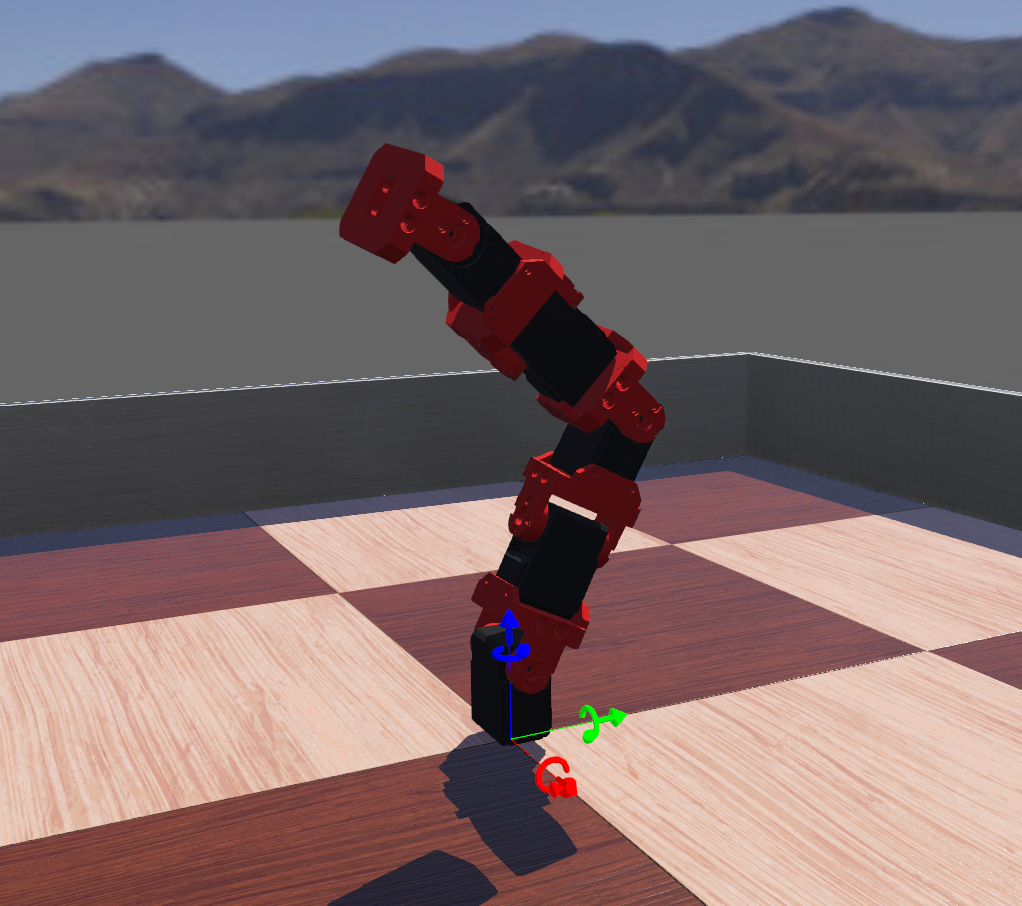
\includegraphics[width=0.8\textwidth]{./Images/webots-robot.png}
    \caption{Modelo virtual do manipulador no Webots.}\label{fig:robot-model}
\end{figure}

\subsection*{Modelagem da Cadeia Cinemática}

A estrutura cinemática do manipulador 5R foi pensada de modo a ser uma simples
cadeia de juntas rotacionais, permitindo uma fácil construção do robô real,
como por exemplo, sendo composto por uma sequência de servo motores conectados
por soquetes como ilustrado na figura~\ref{fig:robot-model}. A cadeia
cinemática é similar ao que já vimos no exemplo dos braço planar 3R, contudo
juntas consecutivas possuem eixos de rotação ortogonais entre si, como indicado na
figura~\ref{fig:kin-chain}. Com isso, a posição do efetuador final não fica 
restrita a um plano perpendicular ao eixo de rotação das juntas, o que permite 
especificarmos no espaço de trabalho,
vetores com três coordenadas para compor a trajetória a ser seguida. Como \(n =
5 \text{ e } m = 3\) o manipulador tem grau de redundância de duas juntas
excedentes. A tabela~\ref{tab:dh-parameters-5r} resume os parâmetros DH
utilizados para modelar a cadeia cinemática.

\begin{table}[htbp]
    \centering
    \begin{tabular}{c c c c c c}
        \toprule
        \textbf{Elo} & \(\theta\)   & \(d\) & \(a\) & \(\alpha\)   \\
        \midrule
        1            & \(\theta_1\) & 0     & 0.06  & \(\pi / 2\)  \\
        2            & \(\theta_2\) & 0     & 0.06  & \(-\pi / 2\) \\
        3            & \(\theta_3\) & 0     & 0.06  & \(\pi / 2\)  \\
        4            & \(\theta_4\) & 0     & 0.06  & \(-\pi / 2\) \\
        5            & \(\theta_5\) & 0     & 0.02  & \(\pi / 2\)  \\
        \bottomrule
    \end{tabular}
    \caption{Parâmetros DH para o manipulador 5R.}\label{tab:dh-parameters-5r}
\end{table}

A fixação de frames imposta pela convenção DH nem sempre permite que o frame da
base do manipulador coincida com o frame do mundo, introduzindo nesse caso a
utilização de \emph{offsets} nos parâmetros variáveis das juntas, ou
transformações fixas entre os frames que não mudam conforme as juntas são
atuadas. Optamos por adotar uma abordagem mais direta, onde introduzimos a
transformação \(\mathbf{T}^{w}_0\) que relaciona o frame do mundo \(\{w\}\) com
o frame da base do manipulador \(\{0\}\):

\begin{equation}
    \mathbf{T}^{w}_0 = Trans_z(0.04) \cdot Rot_z(\pi) \cdot Rot_y(\pi / 2)
\end{equation}

Assim, para se calcular a cinemática direta do manipulador, prosseguimos de
maneira usual na cadeia cinemática adicionando a transformação
\(\mathbf{T}^{w}_0\) ao início da multiplicação matricial:

\begin{equation}
    \mathbf{T}^{w}_5 = \mathbf{T}^{w}_0 \cdot \mathbf{T}^{0}_1 \cdot \mathbf{T}^{1}_2 \cdot \mathbf{T}^{2}_3 \cdot \mathbf{T}^{3}_4 \cdot \mathbf{T}^{4}_5
\end{equation}

Por outro lado, durante a etapa da cinemática inversa diferencial, precisamos
especificar vetores livres \(\xi^w\) que indicam a velocidade cartesiana do
efetuador no mundo em termos do frame da base do manipulador. Para isso,
utilizamos a matriz de rotação da transformação inversa (do frame \(\{0\} \to
\{w\}\)), isto é:

\begin{equation}
    \xi^0 = {Rot(\mathbf{T}^w_0)}^\top \xi^w
\end{equation}

\begin{figure}
    \centering
    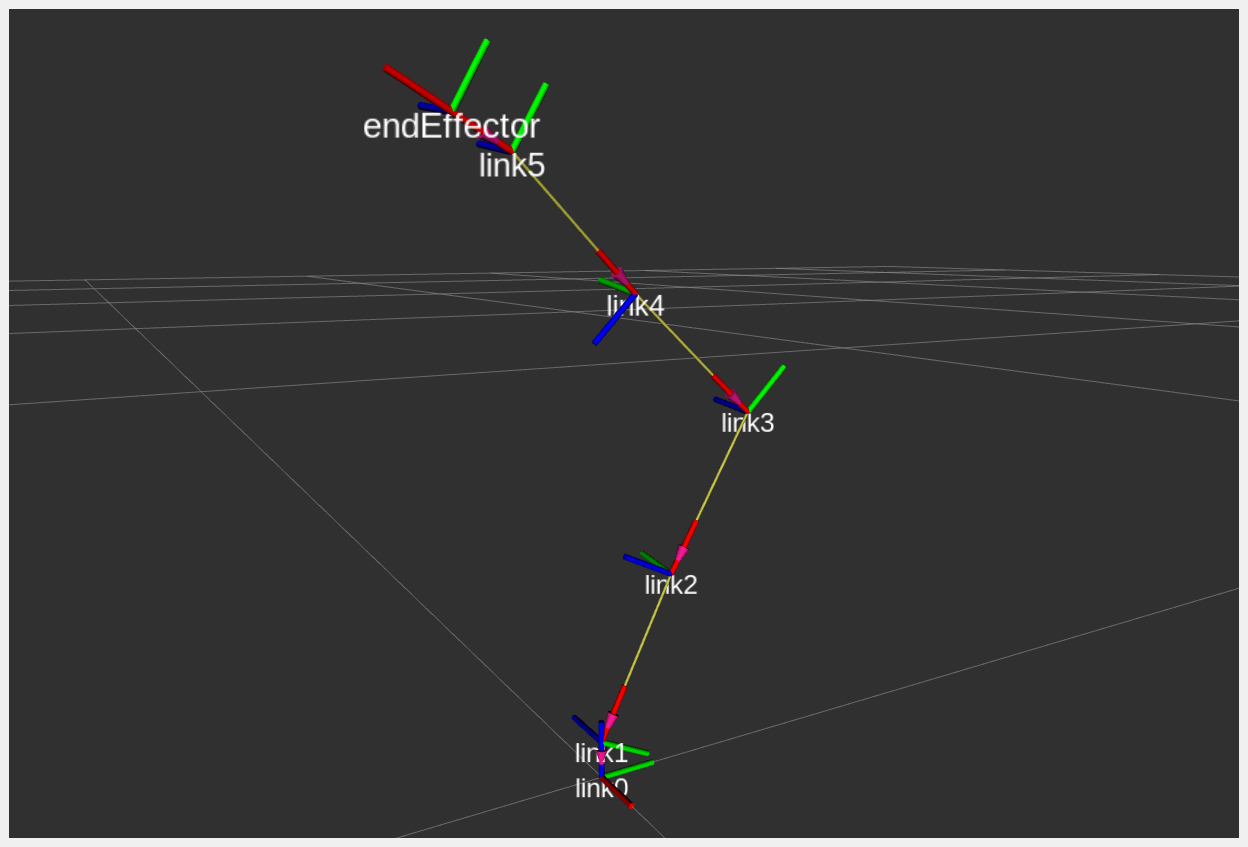
\includegraphics[width=0.8\textwidth]{./Images/rviz-chain.png}
    \caption{Cadeia cinemática visualizada no RViz.}\label{fig:kin-chain}
\end{figure}

\subsection*{Modelo dinâmico do manipulador}

Com o intuito de conferir um caráter mais realista para a simulação, um modelo
dinâmico para o robô foi construído especificando as propriedades físicas e
geometrias de colisão de cada elo no simulador. A figura~\ref{fig:dyn-chain}
mostra as formas primitivas do tipo \emph{Box} (caixas) que foram usadas para
compor a geometria de cada par servo-soquete que compõe um elo da cadeia. Para
o simulador computar o modelo dinâmico ao longo do tempo, foram fornecidas as
informações de massa do servo-motor (disponível na especificação do fabricante)
e no caso dos soquetes, a densidade do material PLA foi utilizada para estimar
sua massa com base no volume da geometria modelada (conjunto de caixas). Além
disso, a definição das matrizes de inércia ficou por conta do próprio
simulador, que estima seu valor com base na massa fornecida e na posição e
orientação das primitivas utilizadas durante a modelagem. Vale ressaltar que a
adição das propriedades dinâmicas tem caráter apenas de aproximação de um cenário
mais real, tendo em vista que o esquema de controle proposto atua apenas na
velocidade das juntas ao passo que a posição do motor é controlada de maneira
automática pelo simulador através de um PID intrínseco à simulação de um
dispositivo como o motor.

\begin{figure}
    \centering
    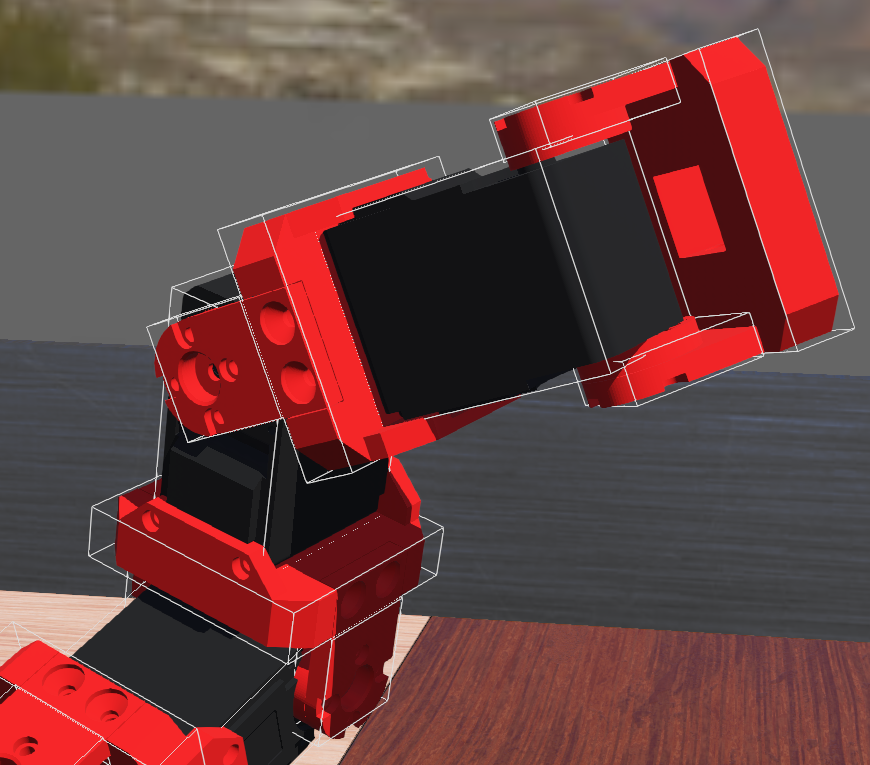
\includegraphics[width=0.6\textwidth]{./Images/dynamic-model.png}
    \caption{Geometria de colisão do modelo virtual do manipulador.}\label{fig:dyn-chain}
\end{figure}

\section{Arquitetura de comunicação}

A comunicação do controlador com o ambiente simulado do robô foi feita através
do uso do framework ROS, que consiste num conjunto de bibliotecas e pacotes de
software que facilitam a troca de mensagens entre diferentes componentes de um
sistema robótico. O próprio simulador Webots oferece suporte nativo ao ROS, com
uma documentação detalhada de como configurar um projeto e o uso básico de
troca de mensagens entre diferentes processos.

A arquitetura de comunicação do ROS é baseada em uma estrutura de grafo, onde
nós representam processos individuais que interagem com outros nós recebendo e
enviando mensagens, através de tópicos. Idealmente, um nó deve ser responsável
por uma única tarefa modular, como controlar os motores do robô ou enviar dados
coletados por um sensor de distância.

Os tópicos são os canais pelos quais os nós trocam mensagens e seguem um modelo
\emph{publisher/subscriber}, onde nós publicam mensagens em um tópico e outros
nós se inscrevem para receber essas mensagens, de maneira completamente
anônima. As mensagens passadas nos tópicos podem variar amplamente e geralmente
são definidas pelo usuário, cobrindo dados de sensores, comandos de controle de
motores, informações de estado, comandos de atuadores entre outros.

\subsection*{Serviços e Ações no ROS}

Serviços e ações constituem outras formas de comunicação entre nós no grafo do
ROS e implementam uma abordagem de troca de mensagens do tipo cliente/servidor.
Serviços representam ações que um nó pode executar com um início e fim
definidos, retornando um único resultado e são normalmente usados para tarefas
que possuem requisição e retorno, como por exemplo capturar uma imagem de um
único quadro, dispensando o processamento contínuo. Por outro lado, ações são
destinadas a tarefas de longa duração e são construídas com base em diferentes
tópicos e serviços. A figura~\ref{fig:ros-action} ilustra as componentes fundamentais
de um nó de ação: um objetivo, um \emph{feedback} e um resultado. Um nó do tipo cliente de ação envia um objetivo
para um nó servidor de ação, que reconhece a requisição, retorna um fluxo
contínuo de dados através de um feedback até que a ação seja concluída ou
cancelada, quando por fim retorna um resultado.

\begin{figure}
	\centering
	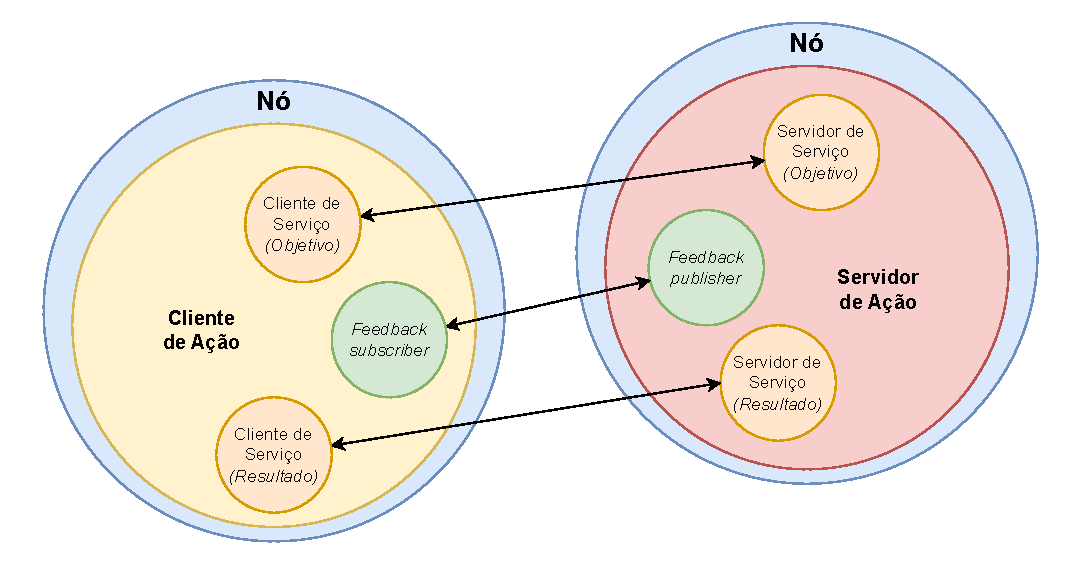
\includegraphics[width=0.8\textwidth]{./Images/ros-action.pdf}
	\caption{Componentes que constituem uma ação dentro do ROS. Adaptado de \cite[p. 36]{bassa_very_2023}.}\label{fig:ros-action}
\end{figure}

\subsection*{Grafo de comunicação no ROS}

Com o objetivo de se executar trajetórias no espaço de trabalho do manipulador,
a arquitetura de comunicação foi projetada de modo especificar um objetivo
através de uma ação do tipo \textbf{trajectory\_action} (nós
\emph{trajectory\_action\_server} e \emph{trajectory\_action\_client}) e
controlar o manipulador (nós \emph{snake\_driver} e \emph{snake\_controller}).
A arquitetura de comunicação proposta para o controle do manipulador é
ilustrada no grafo da figura~\ref{fig:coms_arch}, onde temos nós, tópicos e
ações associados a execução de uma trajetória. A seguir temos uma breve
descrição do funcionamento de cada nó.

\begin{itemize}
    \item \textbf{snake\_driver} {-} Nó instanciado pelo simulador, responsável por controlar os motores do manipulador.
          Está inscrito no tópico \texttt{target\_joint\_states} que recebe a configuração das juntas desejada para o manipulador
          e publica no tópico \texttt{joint\_states} os valores lidos pelos sensores de posição de cada motor. Este nó pode ser substituído por um nó
          que se comunique com um robô real, bastando que a interface de comunicação seja mantida, garantindo uma transferência natural do ambiente simulado para testes físicos.

    \item \textbf{snake\_controller} {-} Nó responsável por implementar a lógica de controle do manipulador. Este nó está inscrito/publica nos dois tópicos
          anteriores para interação com o \emph{driver} do manipulador. Além disso, se inscreve
          num tópico \texttt{rrc\_input}, recebendo parâmetros de controle do algoritmo~\ref{rrc-alg} e publica no tópico \texttt{rrc\_output} dados
          relativos à posição do efetuador final e métricas de desempenho.

    \item \textbf{trajectory\_action\_server} {-} Nó responsável por receber um objetivo de posição e informações do efetuador final para execução de uma trajetória
          no espaço de trabalho do manipulador, publicando no tópico \texttt{rrc\_input} os parâmetros de controle.

    \item \textbf{trajectory\_action\_client} {-} Nó responsável por enviar um objetivo de posição para o servidor de ação \texttt{trajectory\_action\_server} e
          receber o resultado da execução da trajetória. Através da interface de ação, o cliente recebe feedback do progresso da execução da trajetória e o resultado final,
          salvando todos os dados em um arquivo de \emph{log}, para posterior análise.
\end{itemize}

\begin{figure}
    \centering
    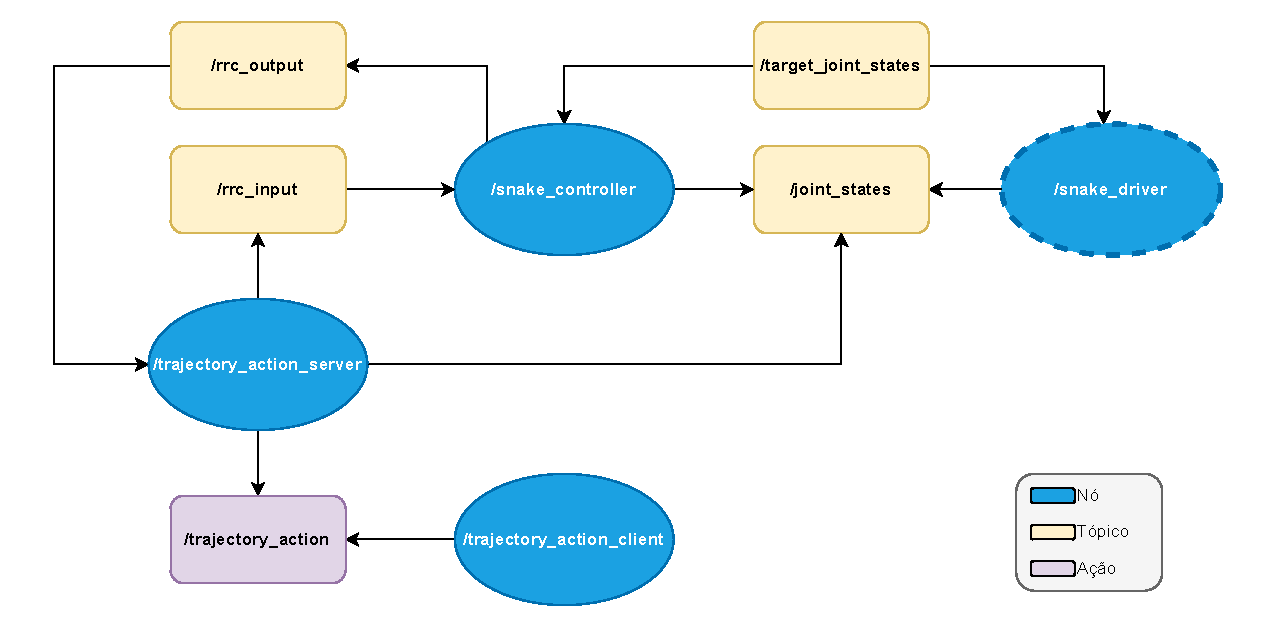
\includegraphics[width=0.8\textwidth]{./Images/ros-arch.pdf}
    \caption{Arquitetura de comunicação proposta para controle do manipulador.}\label{fig:coms_arch}
\end{figure}

\section{O Algoritmo \emph{Resolved Rate Motion Control}}

Para realizar o controle da trajetória do manipulador e também a resolução da
redundância, foi utilizado o esquema de controle \emph{Resolved Rate Motion Control} (RRMC)
definido no capítulo anterior. A figura~\ref{fig:block-diagram} ilustra o
diagrama de blocos do controlador RRMC implementado pelo nó
\emph{snake\_controller}. Dada uma taxa de variação da posição do efetuador
final \(\xi\) e um vetor de velocidades das juntas \(\dot{q_0}\), o controlador
atua atualizando a configuração do manipulador de acordo com a
equação~\ref{eq:pseudo-inverse}.

\begin{figure}
    \centering
    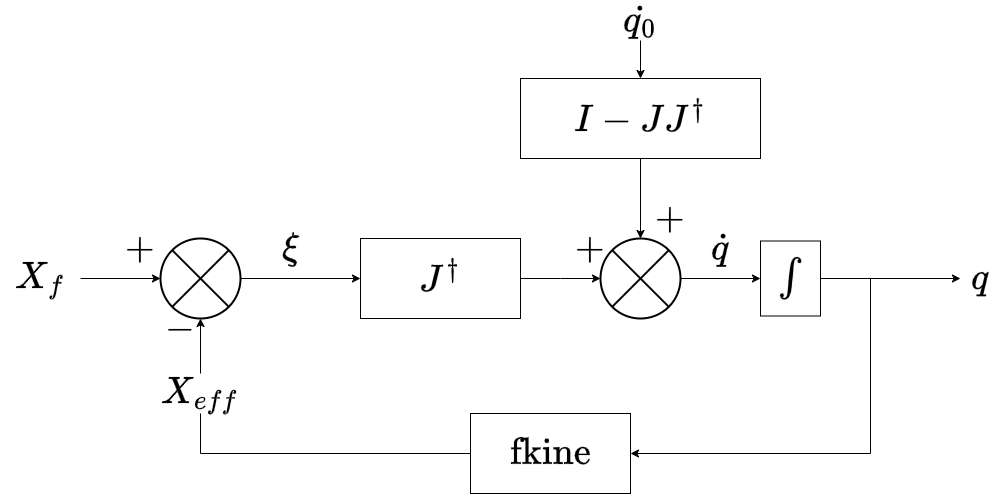
\includegraphics[width=0.6\textwidth]{./Images/control-scheme.png}
    \caption{Diagrama de blocos do controlador RRMC}\label{fig:block-diagram}
\end{figure}

Para a realização das simulações, foi implementado~\footnote{código disponível em 
\url{https://github.com/hugotallys/snakesim}}  o algoritmo~\ref{rrc-alg} que escolhe o vetor \(\dot{q_0}\)
 de acordo com o gradiente dado pela equação~\ref{eq:metric-gradient}. As duas métricas apresentadas anteriormente
foram calculadas: \emph{distância para os limites mecânicos das juntas} e
\emph{medida de manipulabilidade de Yoshikawa}. No primeiro caso, o gradiente é
calculado analiticamente de acordo com a equação~\ref{eq:joint-distance-grad}.
Já para a manipulabilidade, o gradiente é estimado numericamente através de
diferenças finitas, considerando um passo \(h\) suficientemente pequeno.

\begin{algorithm}
    \caption{\emph{Resolved Rate Motion Controller} {-} Atualizando o estado das juntas}\label{rrc-alg}
    \begin{algorithmic}[1]\Procedure{updateJointPosition}{$q$, $\xi$, $k_0$, $\delta_t$, \texttt{metricName}}
        \State$\xi \gets {Rot(\mathbf{T}^w_0)}^\top \xi$
        \State$J \gets Jacobian(q)$
        \State$J^\dag \gets J^\top {(J J^\top)}^{-1}$

        \State$n \gets length(q)$
        \State$\dot{q_0} \gets array(size: n)$

        \For{$i \gets 0 \ \texttt{to} \ n - 1$} \Comment{Calculando o gradiente da métrica}
        \If{$\texttt{metricName} = \texttt{joint\_distance}$}
        \State$q_{mid} \gets 0.5 \times (q_{\max}[i] + q_{\min}[i])$
        \State$\dot{q_0}[i] \gets (-k_0 / n) \times (q[i] - q_{mid}) \div {{(q_{\max}[i] - q_{\min}[i])}^2}$
        \ElsIf{$\texttt{metricName} = \texttt{manipulability}$}
        \State$q_{+} \ , \ q_{-} \gets copy(q) \ , \ copy(q)$
        \State$q_{+}[i] \gets q_{+}[i] + h$
        \State$q_{-}[i] \gets q_{-}[i] - h$
        \State$\dot{q_0}[i] \gets k_0 \times (manipulability(q_{+}) - manipulability(q_{-})) \div (2 \times h)$
        \EndIf{}
        \EndFor{}

        \State$\dot{q} \gets J^\dag \xi + (I - J^\dag J) \dot{q_0}$

        \State\textbf{return} $clipLimits(q + \dot{q} \delta_t, q_{\max}, q_{\min})$ \Comment{Restringe aos limites das juntas}
        \EndProcedure\end{algorithmic}
\end{algorithm}

\subsection*{Simulações}

As simulações focaram na avaliação da resolução de redundância
sob valores variados do ganho (\(k_0\)) e envolveram dois cenários. No primeiro
cenário, o manipulador foi controlado de modo a otimizar a distância para o limite mecânico das juntas, 
executando movimentos internos no seu espaço nulo, mantendo a posição do efetuador final estacionária.
No segundo cenário, além de movimentos internos para otimizar seu índice de manipulabilidade, o manipulador 
seguiu uma trajetória cartesiana entre a posição inicial \(E_i\) e um outro ponto \(E_t\) correspondente à posição desejada
no seu espaço de trabalho. Os índices de desempenho, configuração das juntas e a 
posição do efetuador final foram registrados na simulação de modo a se avaliar 
a eficácia do esquema da resolução de redundância na execução de tais simulações.

Em cada iteração do \emph{loop de trajetória}, o vetor de velocidade é calculado e 
fornecido como entrada para o controlador RRMC. A execução da trajetória para sempre 
que o número máximo de iterações é atingido (em ambos os cenários, definido como 500) ou 
se a norma do vetor de erro de posição se torna menor que 0,01 (apenas no segundo cenário). 
Para avaliar o desempenho em cada trajetória, calculamos a pontuação:

\begin{equation}
	I(w) = \int_0^t {|w(q(\tau))| \ d\tau}
\end{equation}
	
a fim de capturar informações não apenas sobre o estado final da trajetória, mas também ao 
longo de toda a sua execução.

O fluxograma da figura~\ref*{fig:exp-flow} detalha o processo geral para a execução das 
trajetórias do manipulador robótico. Inicialmente, são escolhidas duas configurações 
\((q_0\) e \(q_f\)). Em seguida, calcula-se as posições inicial e desejada (\(E_i\) e 
\(E_t\)) do efetuador final em ambas as configurações. Verifica-se se há colisão com 
o chão (plano $z=0$): caso positivo, retorna-se à escolha das configurações. Se não há 
colisão, escolhe-se um ganho \(k_0\) e calcula-se o erro de posição \(\xi\). Avalia-se 
se há condições de parada da trajetória; se sim, os resultados são salvos e a trajetória 
é reiniciada com um novo ganho \(k_0\). Se não, atualiza-se \(E_i\) conforme o RRMC
e o processo continua até não haver mais ganhos \(k_0\) para escolher, concluindo o 
a execução das trajetórias.

\begin{figure}
	\centering
	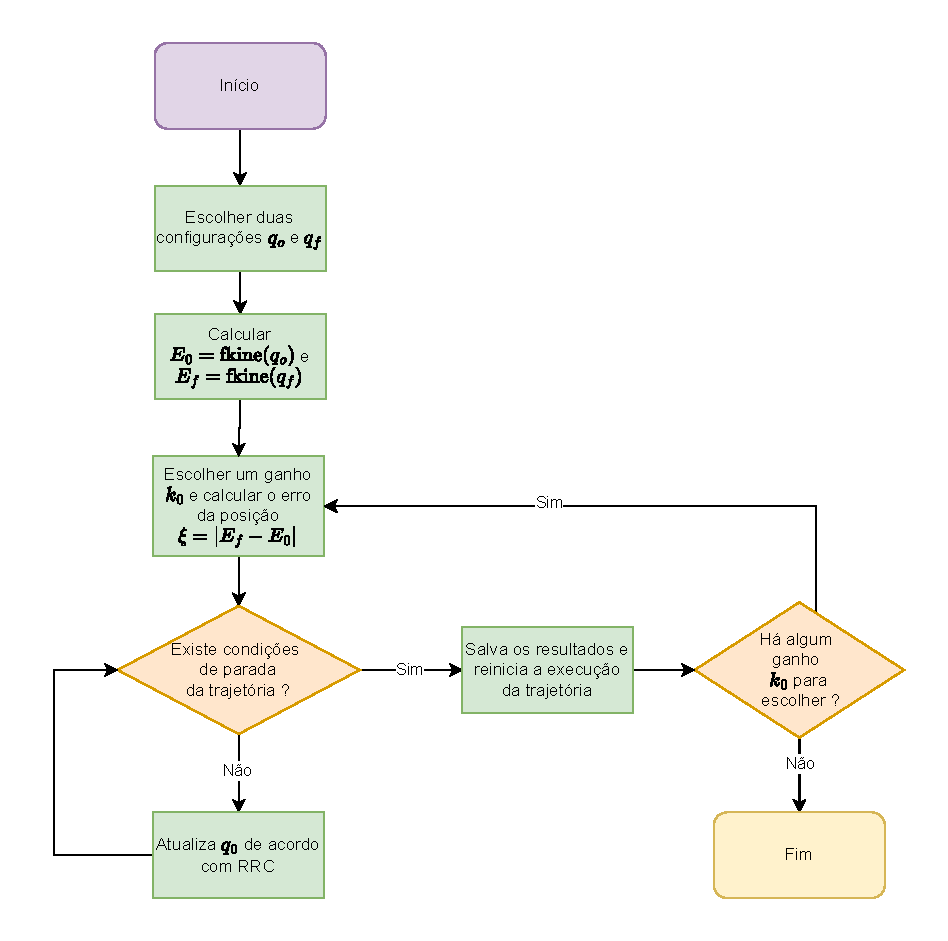
\includegraphics[width=0.8\textwidth]{./Images/exp-flow.pdf}
	\caption{Etapas seguidas na simulação das trajetórias executadas.}\label{fig:exp-flow}
\end{figure}

Vale ressaltar que devido a natureza complexa da determinação do espaço 
de trabalho do manipulador, procurou-se simplesmente escolher 
os pontos inicial e desejado de modo que sejam posições atingíveis no espaço
de trabalho do manipulador, executando-se uma 
trajetória cartesiana na direção do vetor unitário entre os dois pontos.
Além disso, a escolha de tais pontos foi feita de maneira aleatória ao longo de 
diversas simulações, de modo a não privilegiar nenhuma configuração específica do 
manipulador.